\chapter{Introdução}
\section{O que é Diabetes Mellitus?}
O diabetes mellitus(DM) é um doença causada por uma desordem metabólica, caracterizada por hiperglicemia crônica envolvendo distúrbios relacionados à carboidratos, resultado do metabolismo de gorduras e proteínas devido à defeitos na secreção de insulina, ação da insulina, ou ambos. Os efeitos da diabetes mellitus inclui danos a longo prazo, disfunção e falha de vários órgãos. Os sintomas da diabetes mellitus podem ser sede, urinar em excesso, embaçamento da visão e perda de peso. Em caso mais graves, cetoacidose ou um não-cetótica hiperosmolar podendo desenvolver e levar ao estado de consciência ou sensibilidade apenas parcial ou insensibilidade, coma e, na ausência de tratamento eficaz, a morte. Muitas vezes, os sintomas não são graves, ou podem estar ausentes. Os efeitos a longo prazo da diabetes mellitus incluem perda parcial da visão e até mesmo cegueira, nefropatia, que pode levar a insuficiência renal e/ou neuropatia com risco de úlceras nos pés, amputação, incluindo disfunção sexual. Pessoas com diabetes têm um risco aumentado de adquirir doenças cardiovasculares e cerebrovasculares \cite{alberti1998definition}

Segundo \cite{alberti1998definition}, o DM possui duas classificações, Tipo 1 e Tipo 2. A primeira caracteriza-se por ser autoimune que lesa, de forma irreversível, as células do pâncreas, produtoras de insulina e conhecidas como células beta, e seu diagnóstico se dá durante a infância do portador. Enquanto a segunda é consequência da resistência do próprio organismo contra as ações da insulina, o principal fator para se desenvolver essa resistência é a obesidade.

\section{Tipos de Tratamentos Diabetes Mellitus Tipo 1}

As formas de terapias para a diabetes mellitus desenvolveu e mudou bastante desde 1921. Inicialmente as seringas eram a única forma de terapia de injeção de insulina, e até hoje continuam ser o principal método utilizado nos EUA. Os avanços tecnológicos levaram as seringas mais compactas e de diversos tamanhos, e uma ampla variedade de agulhas, ultrafina, microfina e outros sistemas de agulhas. Avanços nos quais aumentaram o conforto dos pacientes.

Toda melhoria de um sistema de administração de insulina possui dois objetivos comuns: conveniência e melhor controle glicêmico. Estudos clínicos demonstraram uma forte relação entre um rígido controle glicêmico e a redução do risco de complicações em pacientes com diabetes mellitus. As principais formas de tratamento são seringas e bomba de infusão de insulina \cite{magnolti2007update}.

\subsection{Seringas}
As seringas dominam o mercado de dispositivos de injeção de insulina. Inicialmente eram grandes, pesadas, tubos de vidros reutilizáveis com um longa agulha que precisava de uma frequente amolação. Seringas de plástico modernas são leves, descartáveis e com agulhas ultrafinas para aumentar o conforto e conveniência dos pacientes. Seringas de insulina são diferenciadas de três maneiras: 

\begin{itemize}
\item Espessura da agulha;
\item Comprimento da agulha;
\item Capacidade da agulha.
\end{itemize}

A maioria dos fabricantes oferecem uma variedade de tamanhos e estilos, estas variações aumentam o conforto e conveniência para o paciente. Sendo essa variedade de produtos a principal vantagem no uso de seringa. Por exemplo, existem seringas fáceis de ler suas medidas, baixas doses disponíveis para aqueles pacientes que têm problemas de visão e que requerem baixas quantidade de insulina. Além disso, os pacientes podem misturar diferentes tipos de insulina em uma seringa para satisfazer as suas necessidades de insulina individuais. Seringas tem alguns inconvenientes. 

\begin{itemize}
\item Carregar um frasco volumosos e seringa pode ser complicado;
\item Podem intimidar muitos pacientes;
\item Técnica de injeção leva tempo e prática para se desenvolver;
\item A manipulação da seringa e o frasco pode ser particularmente difícil para os pacientes com destreza e/ou diminuição da visão;
\item Aplicação de uma dose de insulina e injetando-se com uma agulha e seringa em um ambiente social poderá causar constrangimento.
\end{itemize}

Além disso, a precisão da dose de uma seringa varia com seu tamanho. Estudos mostram que o erro na medição de doses de insulina com menos de 5 unidades foi de quase 10\% \cite{magnolti2007update}.


\subsection{Bomba de Infusão de Insulina}

Bomba de infusão de insulina é um pequeno aparelho eletrônico, do tamanho de um celular ou pager, que está ligado ao corpo do portador da doença por um finíssimo cateter com uma agulha flexível na ponta. Essa agulha é inserida no braço, coxa ou abdômen e deve ser trocada em um período de 2 ou 3 dias. Essa bomba não mede o índice glicêmico ou a quantidade de insulina a ser utilizada, essa medição é feita através do glicosímetro. A Figura ~\ref{fig:bombainfusao}\footnote{\url{http://www.diabetes.org.br/sala-de-noticias/2316-bombas-de-infusao-de-insulina}} representa um aparelho comercial \cite{bode2002insulin}

\begin{figure}[htp]
	\centering
	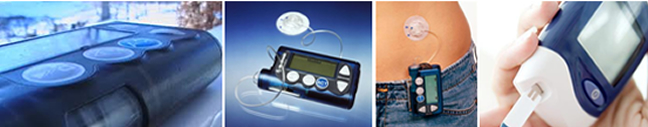
\includegraphics[scale=1]{images/bombainsulina.png}
	\caption{Imagens de uma bomba de infusão de insulina}	
	\label{fig:bombainfusao}
	\cite{portaldiabetes2008}	
\end{figure}


Seu funcionamento é bem simples, libera-se uma quantidade de insulina, programada pelo médico, durante o dia todo, simulando o funcionamento do pâncreas de uma pessoa saudável, entretanto existem cuidados a serem tomados: calcular a quantidade de carboidratos ingeridos a cada refeição e programar o aparelho para injetar uma quantidade de insulina com maior velocidade no organismo nos horário em que se faz as refeições principais.
Quanto a quem pode usar, a pessoa deve cumprir alguns pré-requisitos que são:
\begin{itemize}
\item Conseguir medir o índice glicêmico no mínimo 4 vezes por dia;
\item Durante a fase de adaptação e ajuste da dosagem a serem utilizadas pela bomba, fazer a medição glicêmica de 6 a 8 vezes por dia;
\item Seguir as recomendações médicas além de manter contato e um constante \emph{feedback} com os responsáveis pela bomba e, além de tudo, seguir a dieta recomendada, respeitando quantidades ingeridas;
\item Ter condição financeira para custear o equipamento e o contato com os responsáveis por ele;
\item Estar disposto ao uso da bomba durante o dia todo, 24 horas junto ao corpo;
\item Aprender sobre contagem de carboidratos para saber seu consumo durante as refeições;
\item Praticar exercícios.
\end{itemize}

Cumprindo os pré-requisitos citados temos as vantagens de seu uso que são:

\begin{itemize}
\item Maior flexibilidade no horário das refeições;
\item Se usada corretamente o risco de hipoglicemia é reduzido, e a longo prazo as complicações devido a diabetes também;
\item Melhora o controle glicêmico;
\item Melhora no controle do fenômeno do amanhecer, responsável pelo aumento do índice glicêmico durante a manhã, entre as 4 e 8 horas da manhã, causador da hipoglicemia se o diabético não calculou a dose de insulina antes de dormir, ou não se levantou durante a noite para gerenciá-la.
\end{itemize}

Entretanto mesmo com as vantagens existentes em função de seu uso, caso o diabético seja obeso, ingira grandes quantidades de alimento ou açúcar, ou seja, carboidratos, não praticar atividades físicas, não fazer a medição do índice glicêmico na quantidade de vezes recomendada, ou até mesmo determinar por si só a quantidade de insulina a ser utilizada, essas vantagens deixam de existir.

É importante ter em mente que mesmo com toda facilidade e tecnologia existente o acompanhamento médico não deve ser deixado de lado. As principais indicações médicas para o uso do equipamento são:

\begin{itemize}
\item Fenômeno do amanhecer;
\item Hipoglicemia;
\item Diminuir a variação do índice glicêmico;
\item Hiperglicemia;
\item Recorrente ceatosidade, que é o acumulo de ceatócidos, pois o fígado quebra a gordura e proteína devido à falta de insulina, pois o corpo não consegue utilizar a glicose como energia;
\item Flexibilidade, especialmente para crianças pequenas;
\item Gestação, viagens e atividade físicas;
\item Fobia de injeção;
\item Desejo do diabético \cite{sbc2014, diabetes2013, portaldiabetes2009}.
\end{itemize}

\section{Motivação}
Segundo a Sociedade Brasileira de Diabetes \cite{sbc2014}, diversos estudos realizados mostram que o tratamento feito através da Infusão de insulina tem diversas melhorias quando comparado com outros tratamentos existentes. Entretanto não é o mais utilizado devido ao seu alto custo, devido a importação.
Logo, esse projeto vem com foco social: facilitar o acesso da população brasileira de baixa renda ao equipamento, melhorando sua qualidade de vida dos portadores da doença que se encaixem nesse perfil. 

\section{Objetivos}
Esse projeto tem como objetivo principal desenvolver um software para controle de uma Bomba de Infusão de insulina utilizando o microcontrolador da família PIC - \emph{Programmable Interface Controller} -, PIC18F452. 

\subsection{Objetivos Secundários}

Em segundo plano este trabalho foca em:
\begin{itemize}
\item Aprendizado sobre as características e funcionalidades disponíveis do microcontrolador escolhido;
\item Aprendizado das tecnologias utilizadas como: compilador, simulador e bibliotecas disponíveis;
\item Desenvolvimento das funcionalidades básicas de uma bomba de infusão de insulina;
\item Aprendizado sobre a escolha e uso de um motor de passo;
\item Aprendizado sobre a forma de uso de um \emph{display} de LCD para comunicação com o usuário.
\end{itemize}

\section{Procedimentos Metodológicos}
Inicialmente foi feita uma pesquisa e levantamento bibliográfico sobre o tema em questão para adquirir um melhor entendimento da plataforma, tecnologias e, claro, do problema abordado. Juntamente com essa pesquisa, foi feito um estudo sobre o microcontrolador PIC escolhido, PIC18F452, a partir do material encontrado. O estudo e desenvolvimento foi feito utilizando o compilador MikroC e sua IDE - \emph{Integrated Development Environment} -, já para os testes utilizou-se o simulador Proteus. Em seguida houve-se um levantamento de informações sobre sistemas embarcados, sistemas críticos e sistemas críticos de tempo real, e assim adquirindo-se conhecimento sobre os conceitos de desenvolvimento da área em questão, uma vez que a confiabilidade e segurança do problema proposto é de suma importantância.


O software de controle do protótipo da bomba de infusão de insulina foi desenvolvido na linguagem C, compilado para o microcontrolador já citado, PIC18F452. O sistema é responsável basicamente por gerenciar o perfil de infusão basal, calcular intervalos corretos e passos necessários para uma infusão. Desta forma, o
software foi dividido nos seguintes módulos: Config, LCD, InsulinPump, Motor, Menu, TimerMotor e principal. 

Essa divisão por módulos é, e foi, extremamente importante para o desenvolvimento do sistema. Somando-a à um dos conceitos mais importante desse projeto - OOC, \emph{Object-Oriented Programming With ANSI-C} - são as chaves para a facilidade de manutenção, entendimento do código e possível evolução do projeto.

As responsabilidade dos módulos são bem claras e isoladas:

Config: Centralizar configurações gerais do sistema;
LCD: Abstrair uso do periférico para o resto do sistema;
InsulimPump: Abstrair funcionamento, requisitos de segurança e outras particularidades da bomba;
Motor: Abstrai como se controla o motor e qual tipo está sendo utilizado para infusão;
TimerMotor: Separa o gerenciador de tempo das particularidade únicas do hardware e compilador;
Menu: Facilitar navegação entre menus, simulando máquina de estado;
Principal: Possui o \emph{loop} principal para navegação simples entre os menus existentes.

Os testes do software foram feitos através do simulador Proteus, desenvolvido pela Labcenter. Ferramenta tão importante quanto o OOC para o caminhar deste trabalho. Permite um alto nível de testes, devido a sua facilidade de uso, além do grande auxílio à depuração. O uso do simulador durante o desenvolvimento do software acarreta na minimização dos problemas de integração entre hardware e software, complicações estas que são praticamente impossíveis de estimar. 

E, finalizando, após o desenvolvimento, executou-se uma bateria de testes para se o funcionamento da bomba estava sendo de acordo coma forma especificada, levando em conta toda a integração necessária com os periféricos existentes.

\section{Organização do Trabalho}
\todo{VOLTAR!!!!!!!!!!!!!!!}

A organização desse trabalho tem como início considerações do estudo feito sobre sistemas embarcados, no capítulo \ref{cap:sis_embarcados}. Assunto que abrange definições sobre tipos de sistemas embarcados, componentes como microcontroladores, sensores, atuadores e de interface de comunicações com o usuário. Em seguida, tem-se uma introdução do simulador Proteus, ferramenta de teste utilizada, em conjunto com o compilador. Para complementar as informações sobre o compilador, há uma explicação da organização do microcontrolador escolhido, como pinagem, contadores, barramentos e outros componentes. A partir dessas informações aborda-se o problema proposto, contextualizando-o, descrevendo requisitos e características. 

Após a introdução do problema abordado e explicação de todas as tecnologias utilizadas, vem a descrição e organização do software, explicando cada módulo e forma de implementação. Assim sendo tem-se a discussão de resultados abordando detalhes, motivos e vantagens da implementação para que seja possível finalizar descrevendo a conclusão de todo estudo e projetos futuros.